\section{Theoretische Grundlagen}
\label{sec:theorie}

Im Folgenden wird näher auf einige, für den Versuch notwendige, theoretische Grundlagen eingegangen.

\subsection{Quantenzahlen}

Hier sind insbesondere fünf verschiedene Quantenzahlen von Bedeutung:
Der durch die Nukleonen bestimmte Kernspin mit der Quantenzahl $I$, der Spin mit der Quantenzahl $S$, der Bahndrehimpuls der Isotope mit der Quantenzahl $L$, der Gesamtdrehimpuls mit der Quantenzahl $J$ und die magnetische Quantenzahl $m_J = -J, -J+1, \dots, J-1, J$.
Für einen Zustand mit den Quantenzahlen $(S,L,J)$ lässt sich so über den Gesamtdrehimpuls $J = S + L$ das magnetische Moment
\begin{equation}
    \mu_\text{J} = \mu_\text{B} g_\text{j} \sqrt{J (J + 1)} \,
    \label{eq:magmom}
\end{equation}
definieren, wobei $\mu_\text{B} = \frac{e \hbar}{2 m_e}$ das Bohrsche Magneton und
\begin{equation}
    g_\text{J} = \frac{3 J(J + 1) + S(S + 1) - L(L + 1)}{2 J(J + 1)}
    \label{eq:landefak}
\end{equation}
wie in \cite{Pfeiler2017} den Landé-Faktor darstellt. \\

Die Energiezustände, die das System annehmen kann, sind dabei nicht kontinuierlich, sondern diskrete Zustände.
Wird nun ein äußeres Magnetfeld $B$ angelegt, kommt es zu einer weiteren Aufspaltung, der sogenannten Zeeman-Aufspaltung mit den Energieniveaus
\begin{equation}
    E_\text{mag} = m_\text{J} \mu_\text{B} g_\text{J} B \,.
\end{equation}
Je höher also der Gesamtdrehimpuls $J$ ist, desto mehr zusätzliche Energieniveaus kann das System annehmen.
Darüber hinaus hängen die Niveaus der Aufspaltung auch vom Kernspin $I$ ab.
So kann eine neue Quantenzahl $F = J + I$ definiert werden, die es ermöglicht, über
\begin{equation}
    g_\text{F} = \frac{ F(F + 1) + J(J + 1) - I(I + 1)}{2 F(F + 1)}
    \label{eq:FLande}
\end{equation}
die auch Hyperfeinstruktur genannte Energieaufspaltung
\begin{equation}
    E_\text{hyper} = g_\text{F} \mu_\text{B} B
    \label{eq:hyperfein}
\end{equation}
zu beschreiben.
Ähnlich wie $m_\text{J}$ kann $F$ dabei alle Werte $F = |J - I|,|J-I|+1,...,J+I-1, J + I$ annehmen, die Quantenzahl $m_\text{F}$ ist dann durch $m_\text{F} = -F,\dots, F$ gegeben.

\subsection{Optisches Pumpen}

Mithilfe elektromagnetischer Wellen der richtigen Wellenlänge ist es möglich, in einem Stoff Energieübergänge zu induzieren.
Da diese Wellenlängen bei Rubidium im Bereich des sichtbaren Lichts liegen, wird der Prozess der Anregung auch optisches Pumpen genannt.
Das typische Aufspaltungsschema der hier betrachteten Rubidiumisotope ist in \autoref{fig:rubidiumaufspaltung} dargestellt.
\begin{figure}[H]
    \centering
    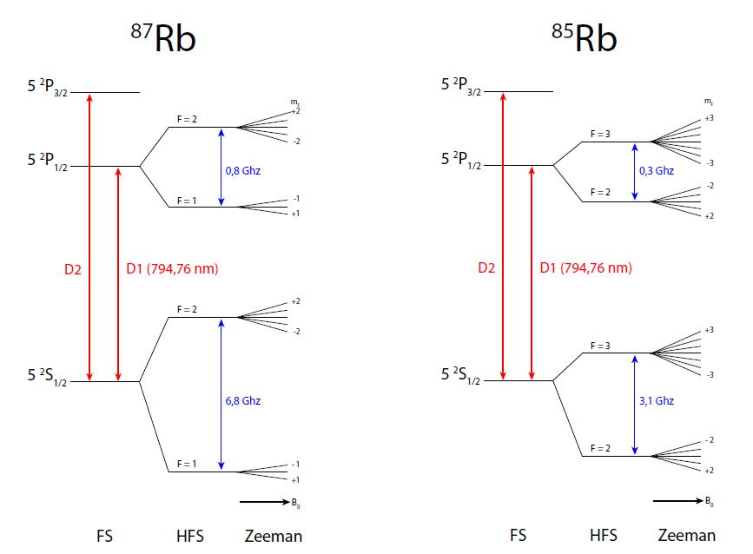
\includegraphics{figures/AufspaltungRubidium.pdf}
    \caption{Feinstruktur- (FS-), Hyperfeinstruktur- (HFS-) und Zeemanaufspaltung der Rubidiumisotope $^{87}$Rb und $^{85}$Rb \cite{rubidiumspalt}.}
    \label{fig:rubidiumaufspaltung}
\end{figure}
Ziel ist es, durch die Wahl der richtigen Wellenlänge und Polarisation möglichst viele Isotope im gleichen Energiezustand zu sammeln.
Dafür wird genutzt, dass je nach Änderung der magnetischen Quantenzahl $m_\text{J}$ beim Übergang zwischen zwei Energieniveaus die Energiedifferenz in Form unterschiedlich polarisierten Lichts absorbiert bzw. emittiert wird.
Ändert sich $m_\text{J}$ beim Übergang nicht, gilt also $\Delta m_\text{J} = 0$, wird linear polarisiertes Licht absorbiert/emittiert.
Dieser Übergang wird als $\pi$-Übergang bezeichnet.
Gilt $\Delta m_\text{J} = \pm 1$, findet der Übergang unter Emission/Absorption von rechts- bzw. linkzirkular polarisiertem Licht statt ($\sigma^\pm$-Übergang).
Hier werden $\sigma$-Übergänge genutzt, um die niederen $s$-Energieniveaus auf höhere $p$-Niveaus zu pumpen.
Von den $p$-Niveaus fallen die angeregten Rubidiumisotope auf das höchste $^2S_{1/2}$-Niveau.
Auch wenn die Isotope von dort aus durch spontane Emission auf ein niedrigeres Energieniveau fallen können, werden sie schnell wieder zurückgepumpt. \\

Durch das Anlegen eines hochfrequenten Feldes lässt sich die Transparenz des Rubidiums beeinflussen.
Liegt die Frequenz genau so, dass
\begin{equation}
    h f_m = g_\text{F} \mu_\text{B} B
    \label{eq:HFFeld}
\end{equation}
gilt, die Hochfrequenzenergie also genau der Energiedifferenz zweier Zeeman-Niveaus entspricht, kommt es, wie in \autoref{fig:trans} zu erkennen zu einem Einbruch der Transparenz.
\begin{figure}[H]
    \centering
    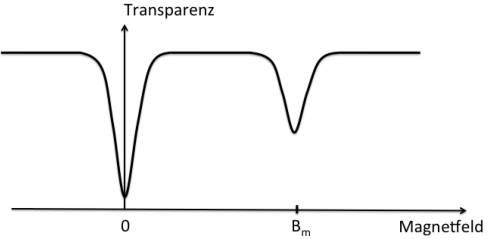
\includegraphics{figures/Transparenz.pdf}
    \caption{Idealisierter Verlauf der Transparenz als Quotient des transmittierten und einfallenden Lichtes in Abhängigkeit der Magnetfeldstärke $B$ \cite{v21}.}
    \label{fig:trans}
\end{figure}
Dieser Einbruch lässt sich durch das Phänomen der induzierten Emission erklären.
Hier werden zwischen vom höchsten Energieniveau der s-Schale durch die HF-Photonen Übergänge ausgelöst, die die Isotope auf niedere Energieniveaus fallen lassen.
Auf den niedrigeren Energieniveaus können die Isotope dann wieder äußeres Licht absorbieren und hochgepumpt werden, die Transparenz sinkt also insgesamt.\\

In der Realität kommt es zu einem zweiten Peak, da Rubidium in zwei natürlichen Isotopen vorkommt.\\

Über den gewöhnlichen Zeeman-Effekt hinaus soll hier auch der quadratische Zeeman-Effekt betrachtet werden, der die Energie um
\begin{equation}
    E_\text{Quad} = g_\text{F} \mu_\text{B} B + g^2_\text{F} \mu^2_\text{B} B^2 \frac{1 - 2 m_\text{F}}{\Delta E_\text{hyper}}
    \label{eq:QuadZee}
\end{equation}
verändert.

Da in diesem Versuch mit Helmholtzspulenpaaren gearbeitet wird, soll hier kurz an die Magnetfeldstärke im Inneren des Spulenpaars, die durch
\begin{equation}
    B = \frac{8 N \mu_0 I}{\sqrt{125} L} 
    \label{eq:Magnetfeld_Helmholtz}
\end{equation}
gegeben ist, erinnert werden.
Dabei bezeichnet $N$ die Windungszahl des Spulenpaars, $L$ den Abstand der beiden Spulen und $I$ die durchfließende Stromstärke.